\chapter{Experimentations et Usages}

\section{Manuel d'utilisation}

\subsection{Préambule}
Notre application a été développée et pensée pour les versions de java supérieures ou égales à la version 8u281.
L'application fonctionne sur Linux avec une interface tournant sur les moteurs graphiques Xorg et Wayland et sur Windows 10.

Les archives jar de Jogl doivent se trouver dans le dossier lib selon le modèle ci-dessous (image)

\info{Nous ne pouvons pas vous garantir si l'application fonctionne sur Mac OS X, aucun des membres de notre n'en possède un.}

\subsection{Lancement de l'application}

Blablabla commande ant run blablabla

\subsection{Utilisation de l'interface utilisateur}

\paragraph{Une fois l'application lancée,} une fenêtre s'affiche \ref{mainframe}. Elle contient une barre de navigation grâce à laquelle vous pouvez ouvrir soit une nouvelle génération, soit une fenêtre d'aide, ainsi qu'un onglet de génération.
\begin{figure}[h!]
    \centering
    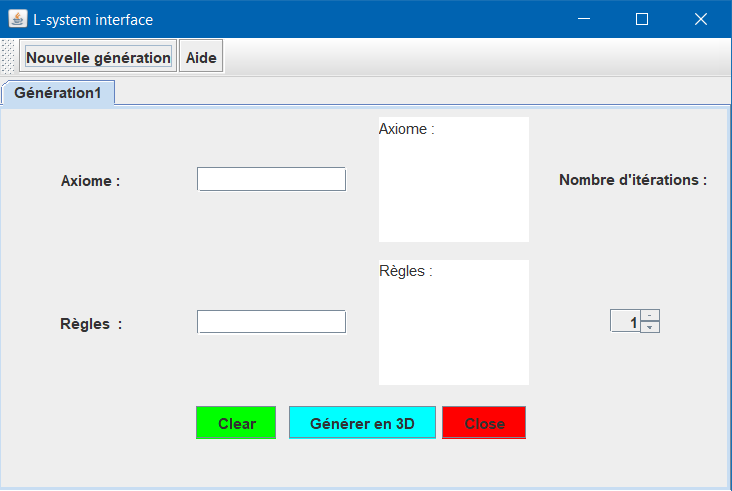
\includegraphics[scale=0.5]{pics/MainFrameGUI.PNG}
    \caption{Fenêtre principale}
    \label{mainframe}
\end{figure}
Il ne vous reste ensuite plus qu'à renseigner votre axiome, ainsi que vos règles et de cliquer sur le bouton \button{Générer en 3D}. Le bouton \button{Close} permet de fermer l'onglet de génération et le bouton \button{Clear} de supprimer votre axiome et vos règles précédemment écrites. Grâce au compteur à droite, vous êtes en mesure de définir le nombre d'itérations de votre génération.

\info{Vous pouvez ouvrir de nouveaux onglets de génération grâce au bouton \button{Nouvelle génération} mais sachez qu'un maximum de trois fenêtres est accepté}

\subsection{Navigation dans l'interface graphique en 3D}
\label{sec:nav_3d}

Pour naviguer dans l'espace 3D, vous pouvez utiliser votre clavier ainsi que votre souris. \info{La souris n'est pas essentielle, le clavier suffit amplement}

\paragraph{Liste des commandes au clavier : }
\begin{itemize}
    \item \textbf{Z} $\xrightarrow{} Avancer$
    \item \textbf{S} $\xrightarrow{} Reculer$
    \item \textbf{Q} $\xrightarrow{} Aller \ à \ gauche$
    \item \textbf{D} $\xrightarrow{} Aller \ à \ droite$
    \item \textbf{A} $\xrightarrow{} Tourner \ la \ caméra \ à \ gauche$
    \item \textbf{E} $\xrightarrow{} Tourner \ la \ caméra \ à \ droite$
    \item \textbf{W} $\xrightarrow{} Prendre \ de \ la \ hauteur$
    \item \textbf{X} $\xrightarrow{} Perde \ de \ la \ hauteur$
\end{itemize}
\paragraph{Liste des commandes à la souris :}
\begin{itemize}
    \item \textbf{Mollette Avant} $\xrightarrow{} Zommer$
    \item \textbf{Mollette Arrière} $\xrightarrow{} Dézoomer$
    \item \textbf{Clic Droit} $\xrightarrow{} Maintenir \ puis \ bouger \ la \ souris \ pour \ changer \ l'orientation \ de \ la \ caméra$

\end{itemize}

\problem{Vous ne pouvez pas utiliser 2 touches ou plus en même temps pour naviguer. Par exemple, enfoncer les touches \textbf{Z} et \textbf{D} pour aller la direction nord-est  est impossible, il vous faut tourner votre caméra dans la direction où vous voulez aller puis appuyer sur \textbf{Z}.}

Fermez la fenêtre 3D pour pouvoir générer un nouveau L-Systeme sans avoir à rouvrir l'application

\section{Tests de notre logiciel}

\subsection{Exemple test 1}

\subsection{Exemple test 2}

\subsection{Possibles problèmes}

Lorsque vous tentez de générer un L-Système, celui-ci est affiché en 3D en utilisant une méthode récursive, si celui-ci est trop long cela peut entraîner une erreur de type StackOverflowError, la fenêtre 3D restera alors blanche, fermer la puis retenter une génération avec moins d'itérations ou tentez une génération avec d'autres règles.

\section{Mesures de performances}

\section{Possibles améliorations}

